\section{Perturbed Minimization}
\label{section:unsorted/perturbed_minimization}

The specific minimization method used in PLOP is a modified version of the TNPACK, truncated Newton minimization package \cite{schlick1992tnpack,schlick1992tnpack2}.
This has been shown to have very good performance on high dimensional minimization problems.
However, as the energy surface of large structures is very rough, having a large number of local minima, simple minimization methods tend to be sensitive to initial conformations, and occasionally small changes in starting conformations, or internal parameters can have a large effect on the final minimized energy, \ref{figure:sensitive_initial_conditions}.
One such approach to many minima problems has been simulated annealing \cite{kirkpatrick1983optimization,vcerny1985thermodynamical}.
However, this performs significantly more sampling, and this requires appreciably more time than a simple minimization method.
Therefore, it is desirable to find a minimization method, which is both somewhat tolerant to local minima and insensitive to initial conformations and quickly arrives upon a solution.
We have performed some initial experiments with such a method.
\begin{figure}
\centering
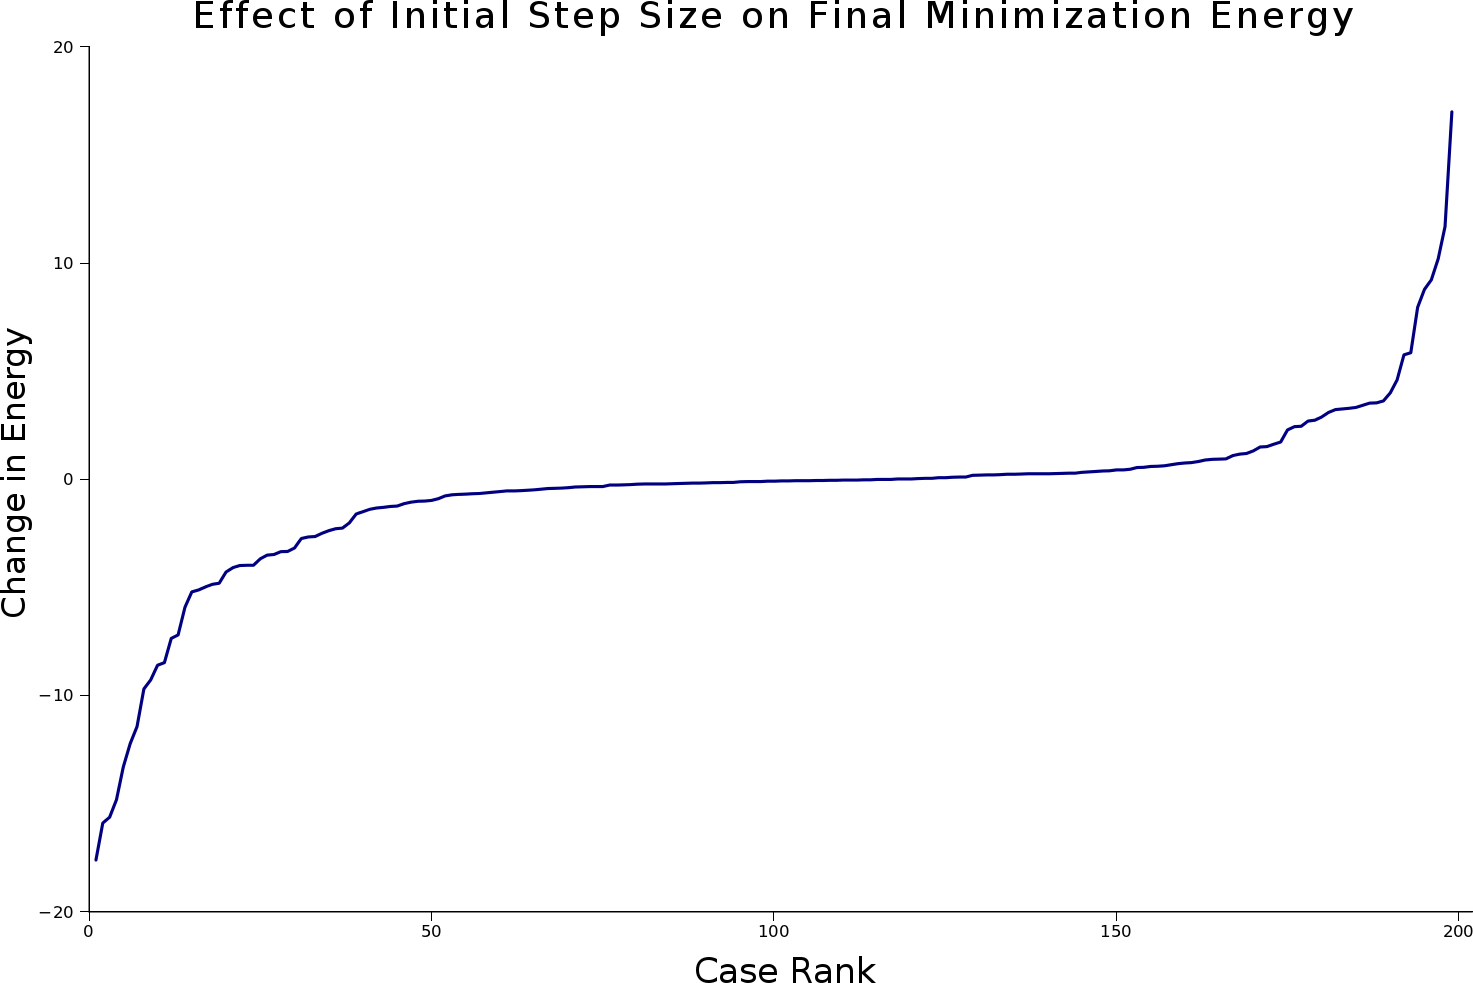
\includegraphics[width=0.8\textwidth,height=0.8\textheight,keepaspectratio]{figures/effect_of_lambda_on_min2.png}
\caption{The effect of varying the initial step size in the line search step of the minimization.
Theoretically this should have little to no effect on the result of the minimization, as the ideal step size would be constant.
It was found that that was not the case, though the effect of the initial guess in the line search seems random.
The cases which were effected to the greatest and least degree showed significant differences in final minimized energy.}
\label{figure:sensitive_initial_conditions}
\end{figure}

\begin{figure}
\centering
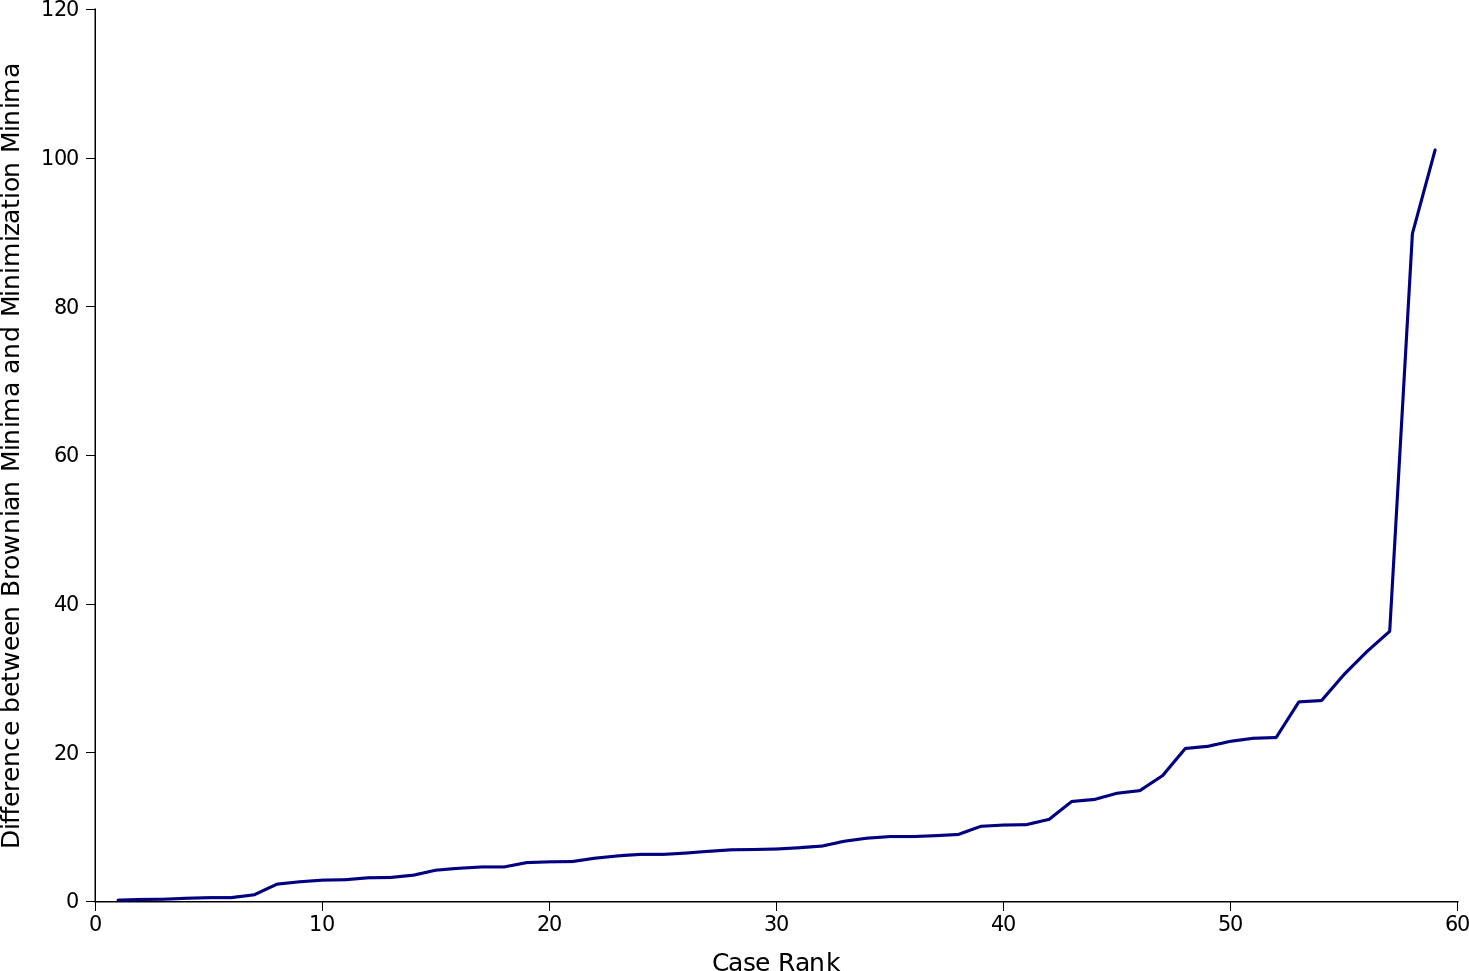
\includegraphics[width=0.8\textwidth,height=0.8\textheight,keepaspectratio]{figures/brownian_sampling.png}
\caption{The difference in minimized energy using the TNPACK truncated newton minimizer and the perturbed sampling routine on a set of 60 small, less than 100 residue, peptides, ordered by rank.
Though for a majority of cases the difference in final energy between a single minimization and multiple perturbed minimization is less than 10 kcal/mol, for approximately 10\% of cases the energy is much higher, up to 60 kcal/mol, far more than the claimed resolution of the current energy model implemented in PLOP.}
\label{figure:brownian_results}
\end{figure}

Our method, perturbed minimization, combines iterative minimization from slightly varied starting conformations with an adaptive stopping rule in order to minimize time spent sampling after finding a reasonably minimum.
The stopping rule, inspired by solutions to the classic game theory secretary problem balances continuing to sample while new lower energy conformations are likely to be found, with efficient stopping after sampling ceases to be productive \cite{freeman1983secretary,chow1964optimal}.

\begin{figure}
\centering
\includegraphics[width=0.7\textwidth,height=0.7\textheight,keepaspectratio]{dot_files/perturbed_minimiztion.png}
\caption{}
\label{figure:perturbed_minimization_flowchart}
\end{figure}

Specifically, the initial structure is perturbed before applying any minimization.
The new perturbed structure is minimized, and if the energy is lower than the current best energy the new low energy conformation along with the energy are saved.
The structure is then reverted to its initial conformation and the procedure is repeated until more than a specified number of steps are performed without finding a new lowest energy structure.
This is effectively the successive non-candidate heuristic solution to the secretary problem applied in reverse (as in this case it is possible to ``call back'' a candidate).
This procedure is described graphically in \ref{figure:perturbed_minimization_flowchart}
This method has been applied to a number of test sets with promising initial results, though it is not clear at the moment in which circumstances this sort of sampling may be necessary.
